\chapter{实现细节}
\label{cha:implementation_details}

\section{原型系统实现概览}
\label{sec:impl_overview}

OpsEvolver 原型围绕工作流编排、故障注入、诊断推理、遥测采集、知识持久化和场景运行六个方面展开实现。与追求复杂分布式调度的工程系统不同，本文更关注研究原型的完整性与可解释性，即首先保证“故障注入、告警形成、诊断分析、经验沉淀”这条链路能够稳定闭合，再在此基础上逐步扩展并发能力、检索能力与评测规模。

\section{多维度故障注入系统}
\label{sec:fault_injection_impl}

\subsection{故障动作注册机制}

系统将故障注入能力统一组织为一组受控动作。不同故障虽然作用层次不同，但都需要满足参数可校验、过程可回收和结果可追踪三项基本要求。这样做的意义在于，离线演化阶段面对的是统一的故障空间，而不必把底层实现差异直接暴露给上层推理流程；与此同时，故障动作也因此能够被约束在可审计、可恢复的安全边界内。

\autoref{tab:fault-actions} 总结了当前原型中已经接入的主要故障动作。

\begin{table}[htbp]
    \centering
    \caption{OpsEvolver 原型支持的故障动作}
    \label{tab:fault-actions}
    \small
    \begin{tabular}{|p{2.4cm}|p{2.2cm}|p{3.0cm}|p{5.0cm}|}
        \hline
        故障动作 & 注入层次 & 关键参数 & 说明 \\ \hline
        ContainerKill & 容器级 & 微服务名、容器名列表 & 使用 Chaos Mesh 杀死指定容器，用于模拟容器崩溃或异常退出 \\ \hline
        PodKill & Pod 级 & 微服务列表、持续时间 & 直接终止目标 Pod，考察编排系统的恢复与上游重试能力 \\ \hline
        PodFailure & Pod 级 & 微服务列表、持续时间 & 让目标 Pod 在一段时间内不可用，用于模拟实例失效 \\ \hline
        NetworkDelay & 网络级 & 微服务列表、延迟、抖动、持续时间 & 通过声明式网络扰动注入链路时延和抖动 \\ \hline
        NetworkLoss & 网络级 & 微服务列表、持续时间 & 注入高比例网络丢包，观察重试和超时行为 \\ \hline
        DeployMisconf & 配置级 & 微服务列表、目标配置项、目标值 & 通过受控修改部署配置模拟资源限制、环境变量等配置失配 \\ \hline
        DiskWoreOut & 内核/宿主机级 & 进程名列表 & 通过内核级故障注入返回 I/O 错误，模拟磁盘故障 \\ \hline
    \end{tabular}
\end{table}

\subsection{基于 Chaos Mesh 的声明式故障注入}

对于容器终止、Pod 失效以及网络扰动等常见云原生故障，本文优先采用 Chaos Mesh 的声明式资源对象实现 \cite{chaosmesh2022}。这类实现方式能够较自然地融入 Kubernetes 的资源管理语义，使故障目标、作用范围和持续时间都具有清晰的外部表示，也便于在演练结束后完成统一回收。

相比直接执行宿主机级别的混沌脚本，声明式注入方式更适合本文所关注的云原生环境。一方面，实验对象与参数能够被完整记录，便于后续复盘；另一方面，不同类型的资源级故障也可以被纳入一致的演练逻辑之中。

\subsection{部署失配与内核级故障注入}

仅依赖 Chaos Mesh 仍不足以覆盖真实运维中常见的配置错误与底层 I/O 异常，因此本文又补充了两类故障。其一是部署配置失配，通过受控修改服务部署参数来模拟资源限制不当、环境变量缺失或启动参数偏差等问题；其二是磁盘 I/O 异常，通过内核级故障注入手段模拟更隐蔽的底层读写错误。与容器级故障相比，这类问题往往更难直接从表面症状判断，也更能检验诊断系统对跨层因果链的理解能力。

\subsection{故障恢复与重复注入控制}

为了保证演练流程的可重复性和环境安全性，系统在每次成功注入故障后都会立即记录注入动作名称、参数和所属周期，并在周期结束后执行恢复逻辑。对于 Chaos Mesh 实验，恢复过程通常表现为删除对应实验资源；对于 Deployment 修改，则需要回写原始 YAML；对于 eBPF 故障，则需要清理内核挂载点或相关映射。

此外，系统会持续维护历史注入记录，以避免重复执行完全相同的故障动作与参数组合。这一机制能够提升离线演化的覆盖效率，使有限的实验预算更集中地探索尚未覆盖的区域。

进一步地，去重逻辑并不只针对“已经尝试过的故障”，也针对“已经尝试但未产生可观测异常的故障”。前者反映系统已经探索过的样本空间，后者反映当前观测条件下暂时难以形成有效信号的区域。将两者同时纳入后续故障选择过程，有助于使离线演化更接近受约束的主动学习，而不是简单的随机扰动。

\section{诊断智能体与动作执行}
\label{sec:diagnoser_impl}

\subsection{Plan-Act-Observe-Reflect 诊断循环}

诊断模块是系统中最核心的推理执行部分。其内部遵循 Plan-Act-Observe-Reflect 循环：首先根据告警和已有上下文生成当前诊断计划；随后从允许动作集合中选择动作并执行；动作完成后将新的观测结果写回上下文；最后根据更新后的证据反思当前假设是否成立，并决定继续搜集证据还是提交根因结论。

当前原型在离线探索和在线推断两个场景中复用了同一诊断引擎，但使用不同的温度和步数上限。探索式诊断侧重多样化线索搜集，因此温度更高；在线推断更强调稳定收敛，因此温度更低、上下文更精简。

\subsection{动作接口设计}

为使诊断过程可控且易于审计，系统将智能体可调用的操作归纳为日志观测、命令执行、指标观测和链路观测四类。日志观测用于读取与目标服务相关的错误信息，命令执行用于获取环境状态与资源信息，指标观测用于识别资源利用和运行状态变化，链路观测则用于分析调用时延传播和错误扩散。不同动作虽然数据来源不同，但都服务于同一目标，即为根因判断提供可比对、可追溯的证据。

动作设计遵循“先汇聚、后分析”的原则，即先把大体量遥测数据整理为更适合诊断的中间结果，再由模型按需利用其中的关键片段。这样既有助于控制上下文长度，也有助于减少原始数据噪声对推理过程的干扰。

\subsection{探索式与推断式两种模式}

离线演化阶段强调探索性，因此系统鼓励模型从应用层、基础设施层、网络层和数据路径等不同视角观察同一告警，以尽可能覆盖多样化的诊断线索。在线场景则更强调收敛速度与稳定性，系统会先检索相似历史案例和可用规则，再在较为精简的上下文中完成推断。换言之，离线模式更重视“多看、多试、多积累”，在线模式更重视“少走弯路、快速定位”。

\subsection{诊断结果评估与成功判定}

相较于论文初稿阶段的概念性描述，当前原型在离线诊断后增加了明确的结果评估步骤。系统会结合已知故障真值，对诊断结论是否真正命中注入故障进行独立判断；当自动评估不足以完成判断时，则辅以启发式的一致性校验。评估结果会被纳入后续历史记录与实验统计之中。

这里需要区分两层含义不同的“成功”。第一层是系统是否在给定步数内形成了完整诊断结论；第二层是该结论是否与真实故障类型和目标组件一致。两者并不等价，因为一条诊断轨迹即使形成了明确结论，也可能由于描述模糊、定位偏差或停留在表面症状而无法通过严格评估。引入这一区分之后，实验分析关注的就不只是“能否给出结论”，还包括“结论是否真正准确”。

\subsection{置信度与证据链提取}

系统在保存诊断结果时，不仅保留最终根因描述，也同步保留置信度与证据链信息，并将诊断过程中的关键观测摘要纳入同一份报告。这样做的意义在于，一方面可以显式区分高置信度和低置信度结论，为后续反馈和复盘提供依据；另一方面也能把模型给出的判断与实际观测到的证据联系起来，从而提升诊断报告的可解释性。

在实验统计中，置信度同样被保留下来，成为分析不同系统中诊断收敛性与知识成熟度的重要信号。

\section{遥测采集与告警生成}
\label{sec:telemetry_impl}

\subsection{AlertGenerator 的监控会话生命周期}

在故障注入成功后，离线演化工作流并不会立即进入诊断阶段，而是先调用 AlertGenerator 在一个受控观察窗口内搜索可观测异常。其默认监控时长为 5 分钟，轮询间隔为 30 秒。系统会在注入完成后的有限时间内持续检查指标、链路和日志，一旦检测到至少一条有效告警，就立即结束监控并进入后续诊断；若直到窗口结束仍无异常，则将该次注入记录为无告警样本。

这种“有限时长、周期轮询、首次命中即返回”的设计首先避免了故障演练阶段长时间占用监控资源，使一次注入对应一个边界清晰的观测会话；同时，它也把离线演化的样本单位固定为“注入后的一段固定观察期”，便于后续历史库与可视化模块做统一统计；更重要的是，它天然支持无告警负样本的保存，因为“没有任何信号被触发”本身就是该会话的有效输出。

在每次监控会话中，系统围绕指标、链路和日志三类遥测信号完成查询。Prometheus 负责提供容器级指标 \cite{prometheus2024}，Jaeger 负责提供调用链信息 \cite{jaeger2024}，日志模块则补充过去窗口内的文本异常线索。三类信号虽然来源不同，但最终都会被整理为统一的告警结果供后续诊断使用。

\subsection{基于指标的异常检测}

指标检测模块主要覆盖容器 CPU、内存、线程和网络等常见运行时指标。系统并不直接把原始时间序列送入大模型，而是先用统计规则把“是否异常”压缩成少量高价值信号。现有实现采用基于历史基线的 $3\sigma$ 检测，对每个候选指标同时计算当前窗口均值和基线窗口统计量。其核心形式可以表示为
\begin{equation}
    \label{eq:zscore-metric}
    z_m(t)=\frac{\mu_{[t-1\text{m},\,t]}(m)-\mu_{[t-12\text{m},\,t-2\text{m}]}(m)}{\sigma_{[t-12\text{m},\,t-2\text{m}]}(m)},
\end{equation}
其中，$[t-1\text{m},\,t]$ 表示注入后最近 1 分钟的当前窗口，$[t-12\text{m},\,t-2\text{m}]$ 表示向前回溯的 10 分钟基线窗口，并刻意留出 2 分钟间隔以减少故障刚发生时对基线的污染。当 $z_m(t) > 3$ 时，系统把该指标视为异常漂移，并进一步映射到统一告警名称，如 \texttt{HighCPUUsage}、\texttt{HighMemoryUsage}、\texttt{NetworkAnomaly} 和 \texttt{HighThreadCount}。

实现上还有一些细节直接影响结果稳定性。系统会显式忽略 \texttt{POD}、空容器名以及 \texttt{istio-proxy}、\texttt{istio-init} 等基础设施容器，避免把 Sidecar 噪声误当成业务异常；与此同时，指标检测并不试图穷举全部 Prometheus 查询，而是优先选择最稳定、最易跨系统复用的容器级指标集。这种取舍虽然牺牲了部分细粒度场景，但换来了在多个微服务基准上更一致的工程行为。

\subsection{基于链路的异常检测}

链路检测模块负责把 Jaeger 中的原始跨度信息转化为服务级摘要。在每次检查中，系统会抓取最近约 10 分钟内的调用链数据，并限制单次读取规模，以避免在复杂系统中无界增长。原始跨度经处理后会保留 \texttt{service\_name}、\texttt{operation\_name}、\texttt{start\_time}、\texttt{duration}、\texttt{parent\_span}、\texttt{has\_error} 等字段，再进一步按服务聚合成 P50、P95、P99 时延、错误跨度数、总跨度数和错误率等统计量。

现有实现主要关注两种链路级异常：一种是高时延，当某服务的 P95 时延超过 1000 ms 时，系统生成 \texttt{HighLatency} 告警；另一种是高错误率，当错误率超过 10\%，且该服务在观察窗口内至少出现 5 个跨度时，系统生成 \texttt{HighErrorRate} 告警。这样的阈值设置一方面过滤掉低流量下的偶发噪声，另一方面也使链路告警能更好地服务于后续根因分析，而不是把每个瞬时尖峰都变成无意义告警。

链路检测对本文尤其重要，因为许多微服务故障并不直接表现为单机资源异常，而是体现为调用树中的等待时间放大、错误在上游链路聚集或某个关键操作的尾时延显著拉长。与指标相比，链路摘要更接近“谁在等谁、谁在失败”的因果结构，因此在 Astronomy Shop 这类追踪信息完备的系统中尤为关键。

\begin{figure}[htbp]
    \centering
    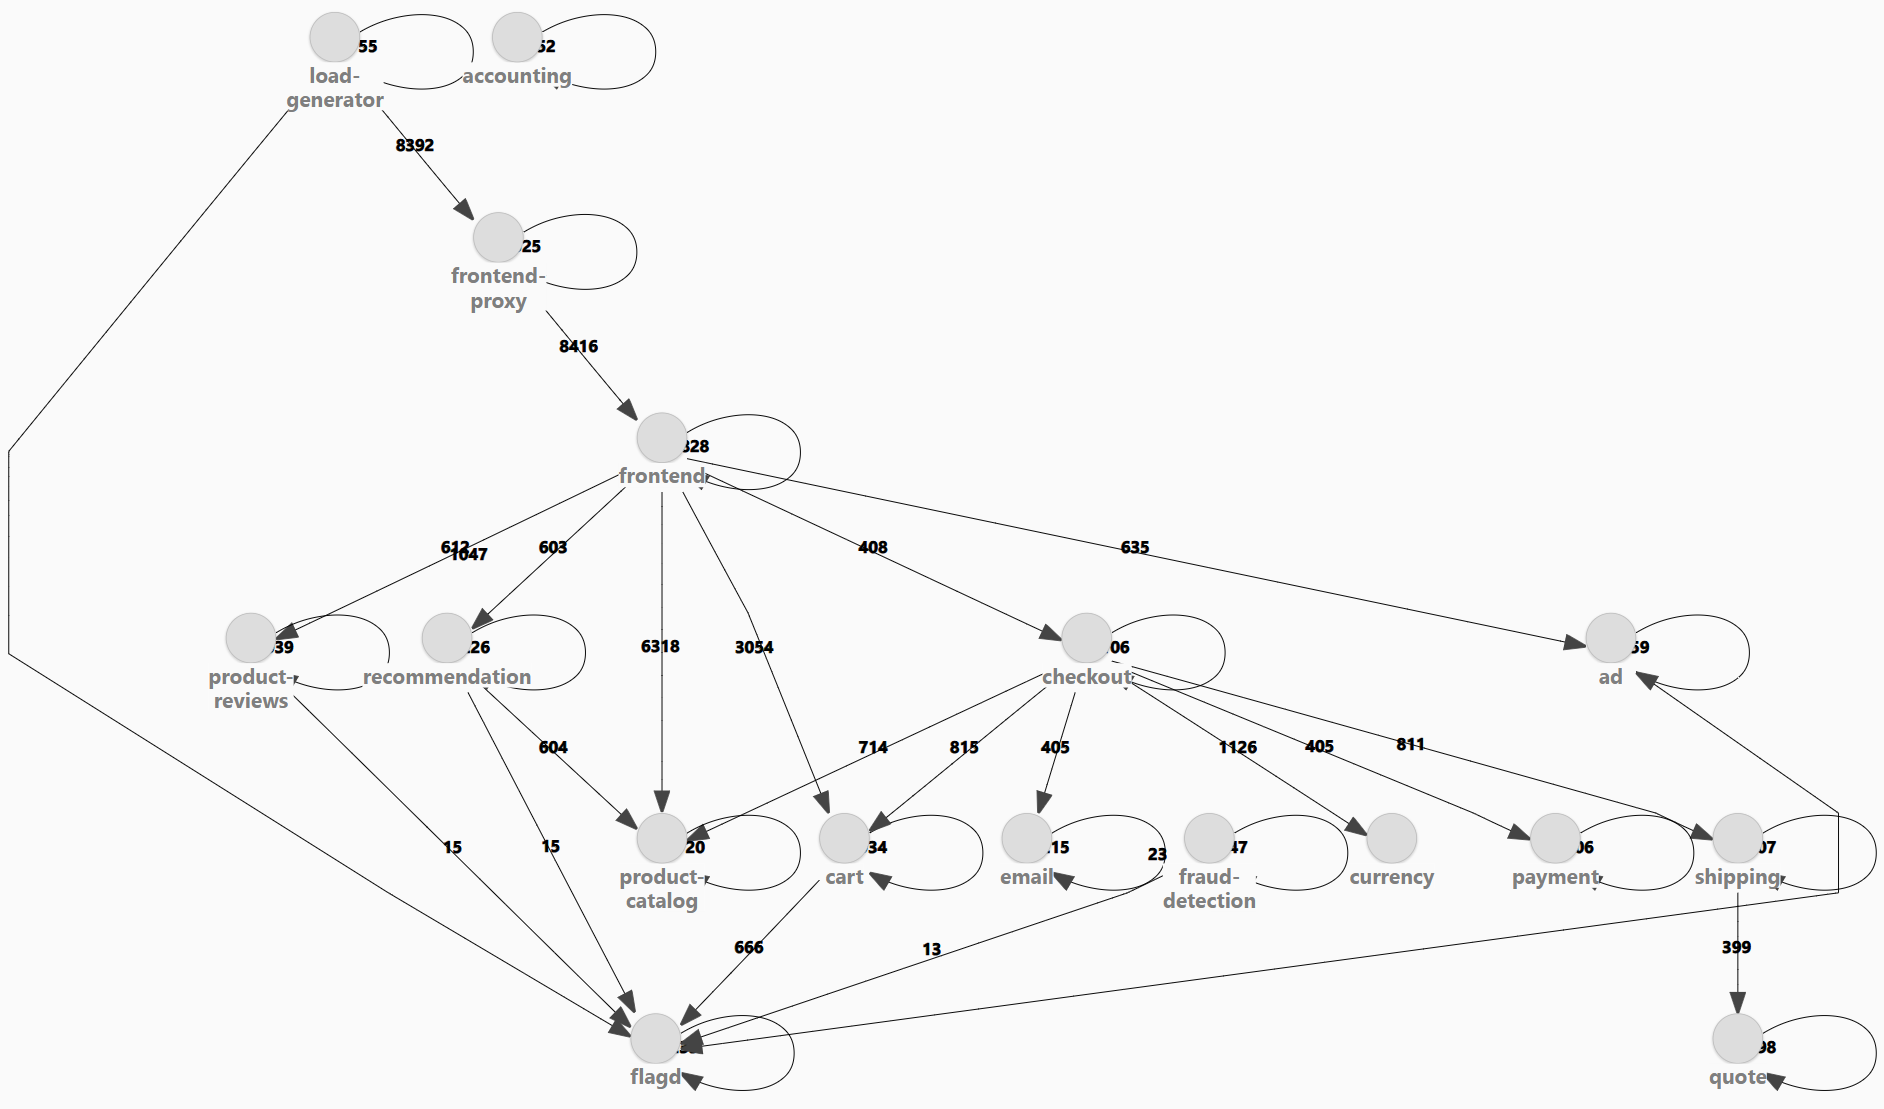
\includegraphics[width=0.7\textwidth]{image/chap03/jaeger-trace-astronomy-shop.png}\\[0.3em]
    \caption{Jaeger 追踪的 Astronomy Shop 调用链}
    \label{fig:jaeger-traces-three-systems-1}
\end{figure}

\autoref{fig:jaeger-traces-three-systems-1} 和 \autoref{fig:jaeger-traces-three-systems-2} 进一步展示了三个系统在 Jaeger 中呈现出的差异化调用结构。Astronomy Shop 呈现出明显的前端扇出结构，适合观察时延在多级依赖间传播；Hotel Reservation 的依赖树更紧凑，利于分析请求失败如何沿前端、搜索和价格服务传导；Social Network 的写路径则具有更深的调用层级和更复杂的中间服务连接，是研究级联故障与上游暴露下游根因的重要场景。

\begin{figure}[htbp]
    \centering
    \begin{minipage}[b]{0.25\textwidth}
        \centering
        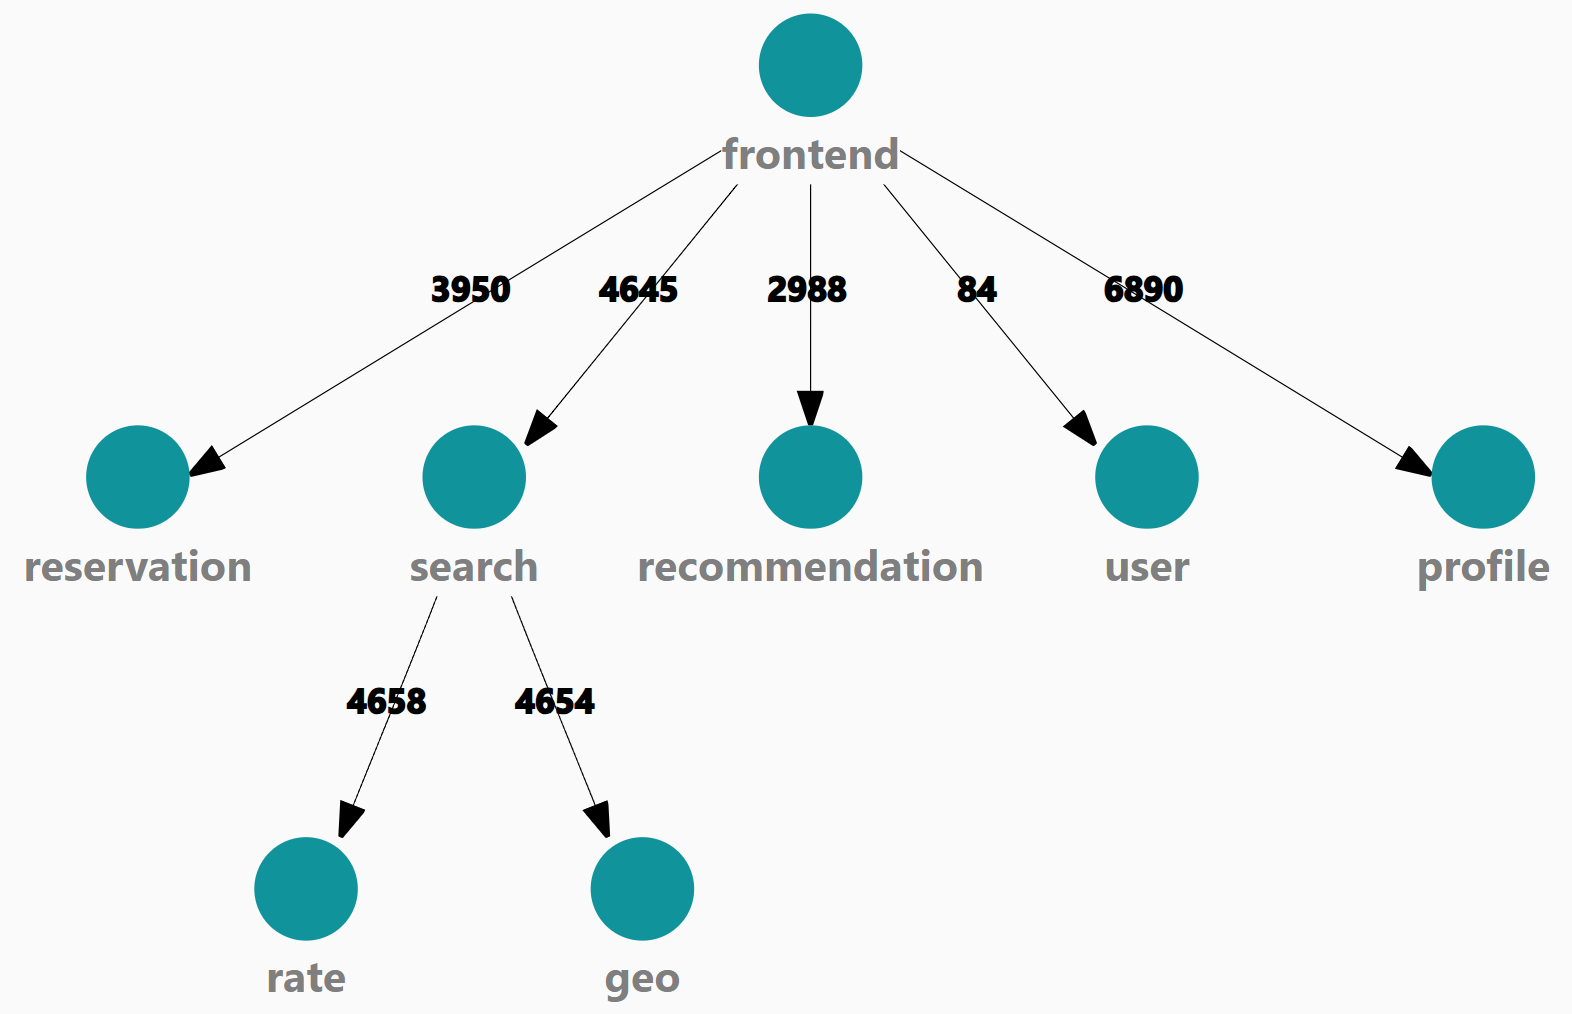
\includegraphics[width=\textwidth]{image/chap03/jaeger-trace-hotel-reservation.png}\\[0.3em]
    \end{minipage}
    \begin{minipage}[b]{0.35\textwidth}
        \centering
        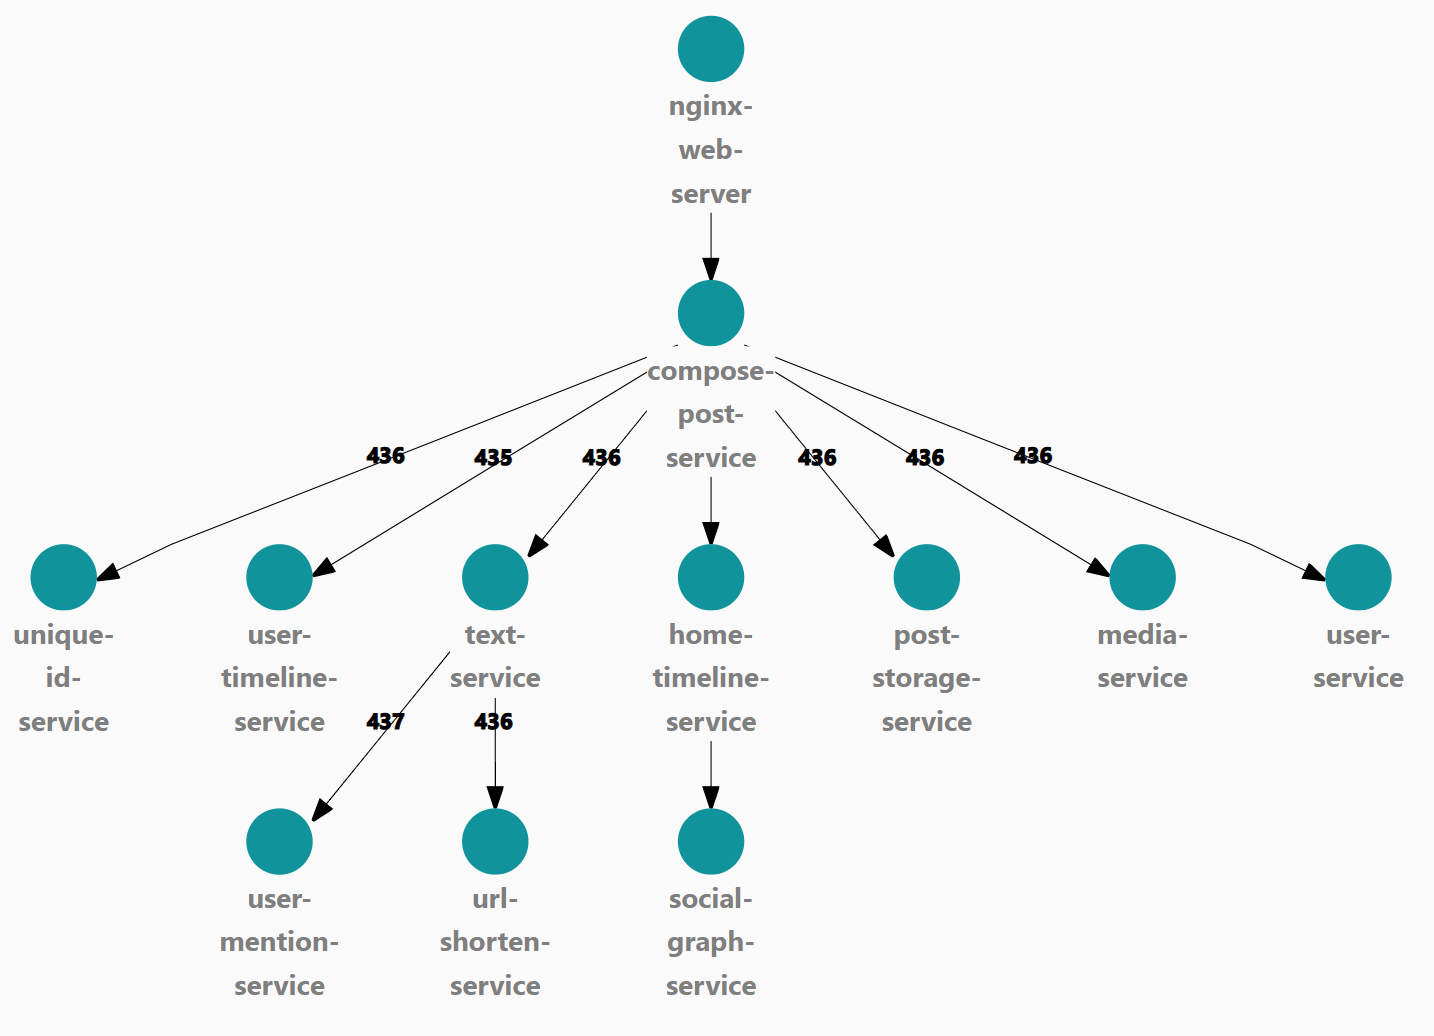
\includegraphics[width=\textwidth]{image/chap03/jaeger-trace-social-network.png}\\[0.3em]
    \end{minipage}
    \vspace{0.8em}
    \caption{Jaeger 追踪的 Hotel Reservation（左）和 Social Network（右）调用链}
    \label{fig:jaeger-traces-three-systems-2}
\end{figure}

\subsection{基于日志的异常检测}

日志检测模块采用“短窗口关键词计数+样本保留”的策略。系统会读取最近 120 秒内与目标命名空间相关的 Pod 日志，并统计错误关键词的出现次数。这种基于关键词与错误模式计数的原型策略，与日志异常检测中常见的经验方法相一致 \cite{he2016experience,yu2024deep}。现有实现关注的关键词包括 \texttt{ERROR}、\texttt{EXCEPTION}、\texttt{CRITICAL}、\texttt{FATAL}、\texttt{FAIL}、\texttt{refused}、\texttt{reset by peer}、\texttt{timed out}、\texttt{deadline exceeded} 和 \texttt{panic} 等。当某个 Pod 在窗口内累计出现至少 3 次错误关键词时，系统生成 \texttt{ExcessiveErrorsInLogs} 告警。

与简单的“只看是否包含 ERROR”不同，本文还会保留错误样本和关键词分布信息，例如错误最集中的服务、出现频率最高的错误模式以及具有代表性的日志片段。这样一来，诊断过程不仅知道“日志异常发生了”，还能够直接利用诸如 \texttt{deadline exceeded}、\texttt{Connection refused} 这类语义线索组织排查路径。

\subsection{统一告警表示}

无论告警来自指标、链路还是日志，系统都会将其整理为统一的告警表示。该表示至少包含告警名称、严重程度、影响服务、数值型证据、拓扑摘要和自然语言描述等信息。统一建模的意义在于，后续诊断过程无需关心告警原始来源，只需要围绕同一语义接口组织排障路径；与此同时，知识库中的症状模式也能够围绕这一统一表示进行检索与匹配。

在监控逻辑上，三类检查按照“指标 $\rightarrow$ 链路 $\rightarrow$ 日志”的顺序轮询执行，但最终返回的是一个统一列表，因此一轮故障演练可能同时包含多种来源的异常。若任一来源检测到有效告警，系统就会认为该轮故障已经进入“可学习区域”；反之则进入无告警集合。从实验结果看，Astronomy Shop 更容易触发 \texttt{HighLatency}，而 Hotel Reservation 和 Social Network 更频繁地表现为 \texttt{ExcessiveErrorsInLogs}。这种跨系统差异，正是统一告警建模之后才能被系统化比较与利用的。

\section{知识库与历史库持久化}
\label{sec:knowledge_base_impl}

\subsection{知识条目表示}

本文以结构化知识条目表示单条可复用运维经验。每条知识围绕症状模式、建议动作、适用条件、置信度、来源信息和产生时间展开，用于回答“看到了什么”“下一步该做什么”以及“这条经验在什么条件下成立”等问题。

这种表示方式与传统 FAQ 或纯文本排障手册不同，它既服务于人类阅读，也服务于机器检索与上下文组装，因此能够在后续诊断中被直接引用，并在反馈环节中被修正或降权。

\subsection{知识库存储与更新}

知识条目与规则库均采用外部持久化方式保存。每完成一轮离线演化，系统都会把新产生的知识与规则追加到长期记忆中，使环境经验能够随演练持续累积。本文原型尚未引入更复杂的语义检索基础设施，而是优先采用便于审查和复盘的轻量级持久化方式，以满足原型验证阶段的研究需求。

\subsection{历史记录与可追溯性}

除知识库外，系统还专门保存逐轮演化历史，用于记录注入事件、告警快照、诊断轨迹摘要、生成的知识条目以及规则集合。同时，对于“成功执行但未产生任何可观测告警”的故障注入，系统也会单独保留记录，以便后续分析可观测性边界。

与只保存最终根因不同，这种历史记录方式使研究者能够回答如下问题：某条知识是在哪一轮演化中生成的；哪种故障注入最容易产生高价值知识；某次失败诊断究竟败在检索、规则还是观测数据不足；哪些故障在当前工作负载和观测窗口下难以形成有效样本。第四章中的有效注入率、无告警分布以及故障-告警关联分析，均建立在这些持久化记录之上。

\section{实验分析数据管线}
\label{sec:analysis_pipeline}

为了将原始历史记录转化为论文中的统计结果，本文构建了一条独立于核心工作流的分析管线。其核心思路是将逐轮历史记录与知识库快照整理为统一的周期级样本表，再围绕这些样本表生成统计图和分析结果。

\subsection{逐周期样本表构造}

在实验分析阶段，系统首先将不同基底模型、不同命名空间下形成的历史记录与知识快照统一整理为周期级样本表。每一条样本对应一轮有效演化，记录故障类型、目标服务、告警数量、告警模式、诊断结果、置信度、严格评估结果、诊断步数以及该轮新增知识和规则等信息。这种“以周期为单位”的样本表示方式，使离线演化实验可以被视为一个随时间逐步展开的数据集，从而便于进行横向比较与纵向观察。

\subsection{统计图与分析维度}

基于上述样本表，本文进一步围绕故障分布、诊断结果、知识时间线、故障与服务覆盖热力图、故障到告警的关系图、知识置信度以及无告警样本分布等维度开展统计分析。这些分析过程并不改变核心诊断逻辑，而是为实验部分提供了一套能够反复复用的观察视角。特别是对无告警样本的单独统计，使过去在实验中容易被忽略的“负样本”也能够进入统一分析框架。

从研究方法上看，这意味着 OpsEvolver 不仅能“运行实验”，还具备将实验结果结构化、可视化和可对比化的能力。对于后续扩展更大规模实验、做版本间对比或加入新的被测系统，这一点尤为重要。

因此，完整的历史记录机制是支撑系统复盘、去重和未来量化评估的重要基础。

\section{实验场景部署与工作负载驱动}
\label{sec:scenario_impl}

为验证框架在不同业务特征下的适用性，原型接入了多个典型微服务应用场景，包括 Hotel Reservation、Social Network、Astronomy Shop 和 Train Ticket。不同应用都被统一纳入同一实验流程，在部署完成后自动进入工作负载驱动阶段，并在实验结束后完成环境清理。

在工作负载设计上，Astronomy Shop 使用系统自带的持续流量组件；Hotel Reservation 与 Social Network 则通过周期性外部压测持续维持业务请求。后两者采用按分钟触发的 CronJob 方式组织工作负载，单次请求阶段持续约 50 秒，并结合较小的连接规模和指数分布到达过程，以保证注入窗口内既有稳定流量，又不会让相邻两轮压测完全重叠。

更具体地说，Hotel Reservation 主要施加中等强度的混合查询与预订流量，Social Network 则主要驱动发帖相关写路径。两者虽然业务请求模式和压测强度不同，但都遵循统一的“周期性触发、持续施压、保留空档”的调度结构，从而使告警生成器能够在故障注入后的观察窗口内持续看到业务调用对异常的放大效应。

场景层的统一封装带来的直接收益是：核心工作流无需感知不同系统的部署差异和流量来源，只需依赖统一的场景接口即可完成演练。这也为后续扩展更多基准系统提供了稳定边界。

\section{本章小结}
\label{sec:chap03_summary}

本章从故障注入、诊断引擎、遥测采集与告警生成、知识持久化、分析数据管线以及场景部署等方面介绍了 OpsEvolver 的具体实现。可以看到，系统并不是单纯围绕 LLM 组织，而是将大模型能力嵌入到故障演练、环境交互和知识管理的整体工程流程中。基于这些实现，下一章将进一步分析该原型在实验对象、能力覆盖和典型案例上的表现。
